
\documentclass[a4paper, oneside, 11pt]{report}
\usepackage{epsfig,pifont,float,multirow,amsmath,amssymb}
\newcommand{\mc}{\multicolumn{1}{c|}}
\newcommand{\mb}{\mathbf}
\newcommand{\mi}{\mathit}
\newcommand{\oa}{\overrightarrow}
\newcommand{\bs}{\boldsymbol}
\newcommand{\ra}{\rightarrow}
\newcommand{\la}{\leftarrow}
\usepackage{algorithm}
\usepackage{algpseudocode}
\usepackage{natbib}
\usepackage{rotating}

\topmargin = 0pt
\voffset = -80pt
\oddsidemargin = 15pt
\textwidth = 425pt
\textheight = 750pt

\begin{document}

\begin{titlepage}
\begin{center}
\rule{12cm}{1mm} \\
\vspace{1cm}
{\large  CMP-7009A Advanced Programming Concepts and Techniques}
\vspace{7.5cm}
\\{\Large Project Report - 16 January 2020}
\vspace{1.5cm}
\\{\LARGE Simulating the activities of an Ant colony}
\vspace{1.0cm}
\\{\Large Group members: \\ Alvin Lu}
\vspace{10.0cm}
\\{\large School of Computing Sciences, University of East Anglia}
\\ \rule{12cm}{0.5mm}
\\ \hspace{8.5cm} {\large Version 1.0}
\end{center}
\end{titlepage}


\setcounter{page}{1}
%\pagenumbering{roman}
%\newpage


\begin{abstract}
Ants have always been a popular animal that was researched for it's behaviour. Findings from it has benefited areas such as machine learning, algorithm discovery and server optimisation. This project aims to create a realistic ant simulator that can be used be researchers and educators to discover potential behaviours or run simple simulations for demonstrations and research. It used an intelligent ant path-finding algorithm that utilises surrounding pheromone data, distance from hive and individual memory. The result was an Ant simulator that provides customisation of various environmental and ant values that can be controlled at the users pace. The software is flexible, replicable and portable which promotes future expansion and reuse.
\end{abstract}

\chapter{Introduction}
\label{chap:intro}

The biological world has always been a source of inspiration for computer models and algorithms. Within successful model developed, swarm intelligence have always been a topic of interest spanning across wide range of disciplines \citep{Swarm_Intro}. In computing, swarms are usually associated with ants that exhibits large amount of behaviours that can potentially be used to optimise algorithms. Whilst there exist techniques and simulations \citep{Ant_Simulator} \citep{Ant_Simulator_Revisited} \citep{Ant_Simulator_Intro}  that mimics the certain behaviour of ants, there aren't software available that simulate ants realistically in  the biological world.

This project aims to develop a realistic ant simulator that allows customisation of various biological settings to simulate different ant colonies in varying environments. It will provide a method to show an accurate representation of ant behaviours, simulate survivability or ants in different settings, and reveal emergent properties that may benefit future swarm intelligence.

\section{Report structure}
Chapter \ref{chap:intro} will provide an introduction to the topic which will be followed by chapter \ref{chap:background} that provides scientific background, previous materials and motivation of for the project. Chapter \ref{chap:design} will detail the design considerations for the solution, supported by analysis of previous literature and existing solutions. Implementation details will be explained in chapter \ref{chap:Implementation} showing figures of the solution and design modifications made. Chapter \ref{chap:Testing} will provide testing and evaluation of the final software with discussions on it's strengths and weakness will be provided in chapter \ref{chap:discussion}. The report will the be summarised within chapter \ref{chap:conclusion} providing a conclusion to the project.

\chapter{Background}
\label{chap:background}
\section{Background information}
Swarming is a behaviour that is commonly found in social animal species \citep{Swarm_Animals}. The concept of swarming is having a large group of individually operating unit (agents or individual animal) working together to achieve a task that is typically to great for a unit to complete on its own \citep{Swarm_Explanation}. Large amount of research has been conducted to explain the evolutionary benefits of such behaviour and researchers are aiming to adapt some of these properties into various computer systems. This is commonly achieved by having a group relatively simpler agents that can communicate between each other instead of a singular system to complete tasks collectively by converging individual accomplishments \citep{Swarm_Properties}.

Within animals that exhibit swarming, ants are one of the insect that has been vigorously studied for their behaviour. Ants most commonly utilise swarming during the process of foraging. Certain species of ants are shown to leave pheromones to share information an individual ant has learnt \citep{Ant_Pheromones}. The two most common pheromones are home pheromones that can guide them home and also pheromones that guide other ants to food sources \citep{Ant_Pheromones}. The pheromones can vary in their duration and potency, which allows transfer of information such as recency and importance of the information \citep{Ant_Pheromones}. Ants are also shown to retain memories of places it has seen, using visual cues to guide them to their destination \citep{Ant_Memory_1} \cite{Ant_Memory_2} \cite{Ant_Memory_3}. Within certain species of ants, they are shown to have extra ways to find their ways such as using polarized light \citep{Ant_Navigation_Light}, magnetic \citep{Ant_Navigation_Magnetic_1} \cite{Ant_Navigation_Magnetic_2} and sun \citep{Ant_Navigation_Wind} compass.


\section{Existing methods}
Currently, an ant simulator was found publicly available online that uses the MASON simulation toolkit \citep{Mason}. The simulator provides a list of features listed below:
\begin{itemize}
	\item Allows customisation of certain values such as the ant population and evaporation rate.
	\item Allows pausing, playing and speeding up or slowing down the simulation.
	\item Shows the pheromone and ant data of a particular point in the map when clicked
\end{itemize}

The simulator provides quick and easy way to visualise movements of the ants however it the customisation was limited as the location of the hive, food and obstacle type can not be changed. This simulator aims only to show how ants eventually converge into a path from hive to food shown in figure \ref{fig:MASON_Ant_Converged} which limits the flexibility of the simulator. The source code of the ant simulator is available on \textit{GitHub} for reference.

\begin{figure}[htb]
	%\begin{center}
	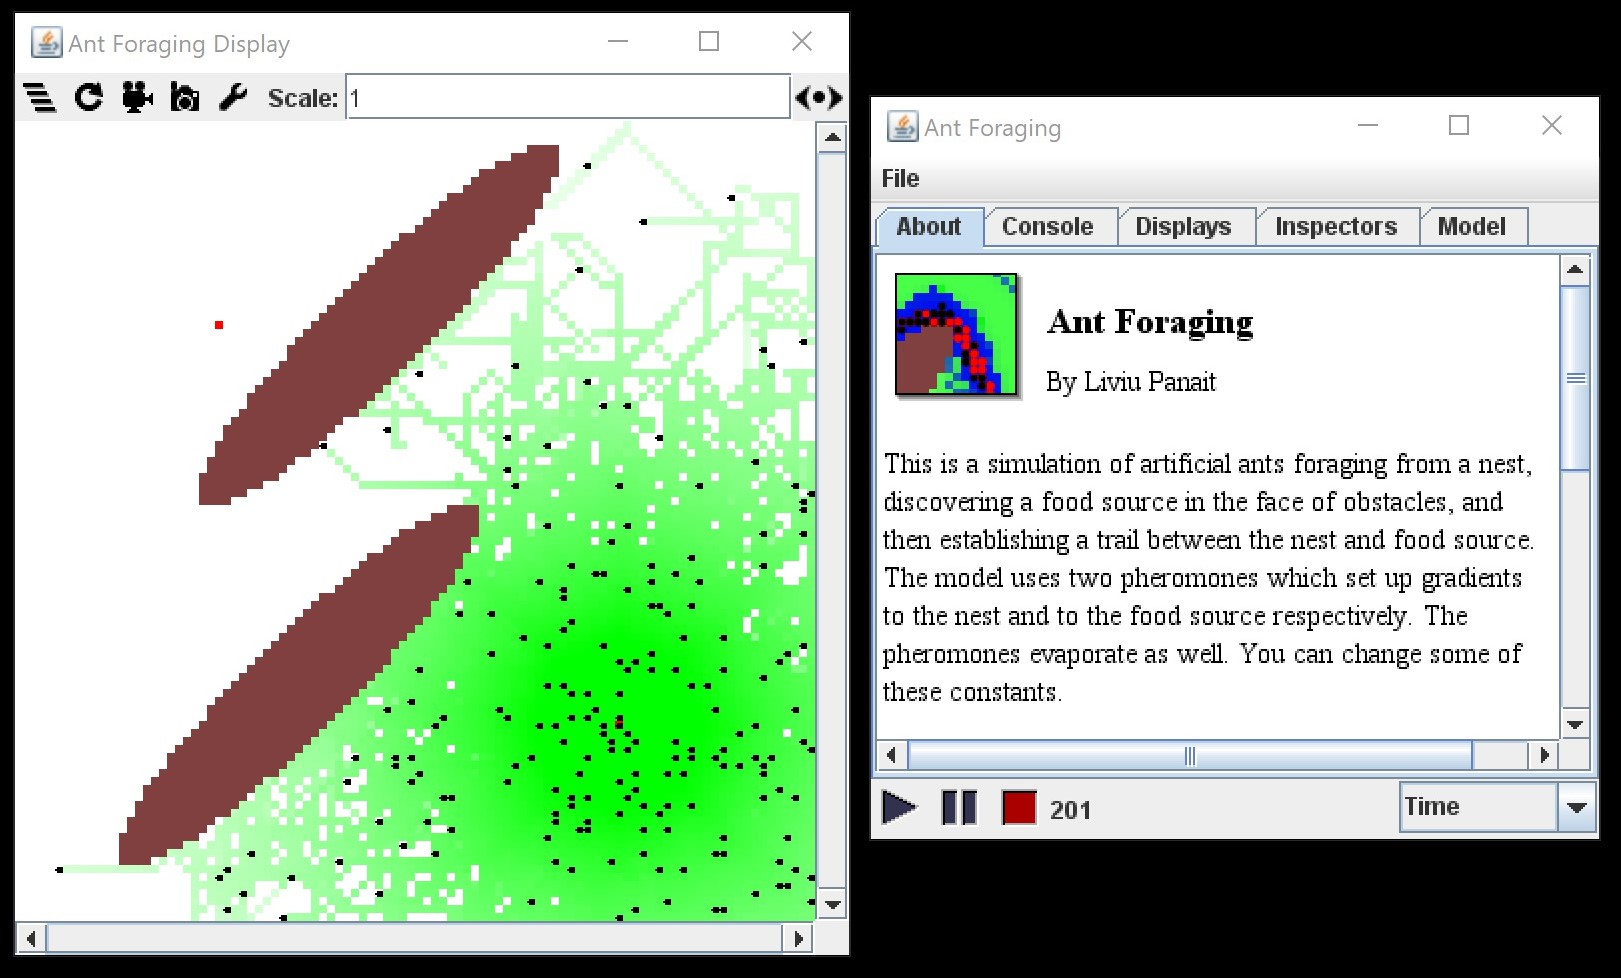
\includegraphics[width=1.0 \columnwidth]{MASON_Ant.jpg}
	\caption{Ant simulator developed by Liviu Panait \citep{Ant_Simulator}}
	\label{fig:MASON_Ant}
	%\end{center}
\end{figure}

\begin{figure}[htb]
	%\begin{center}
	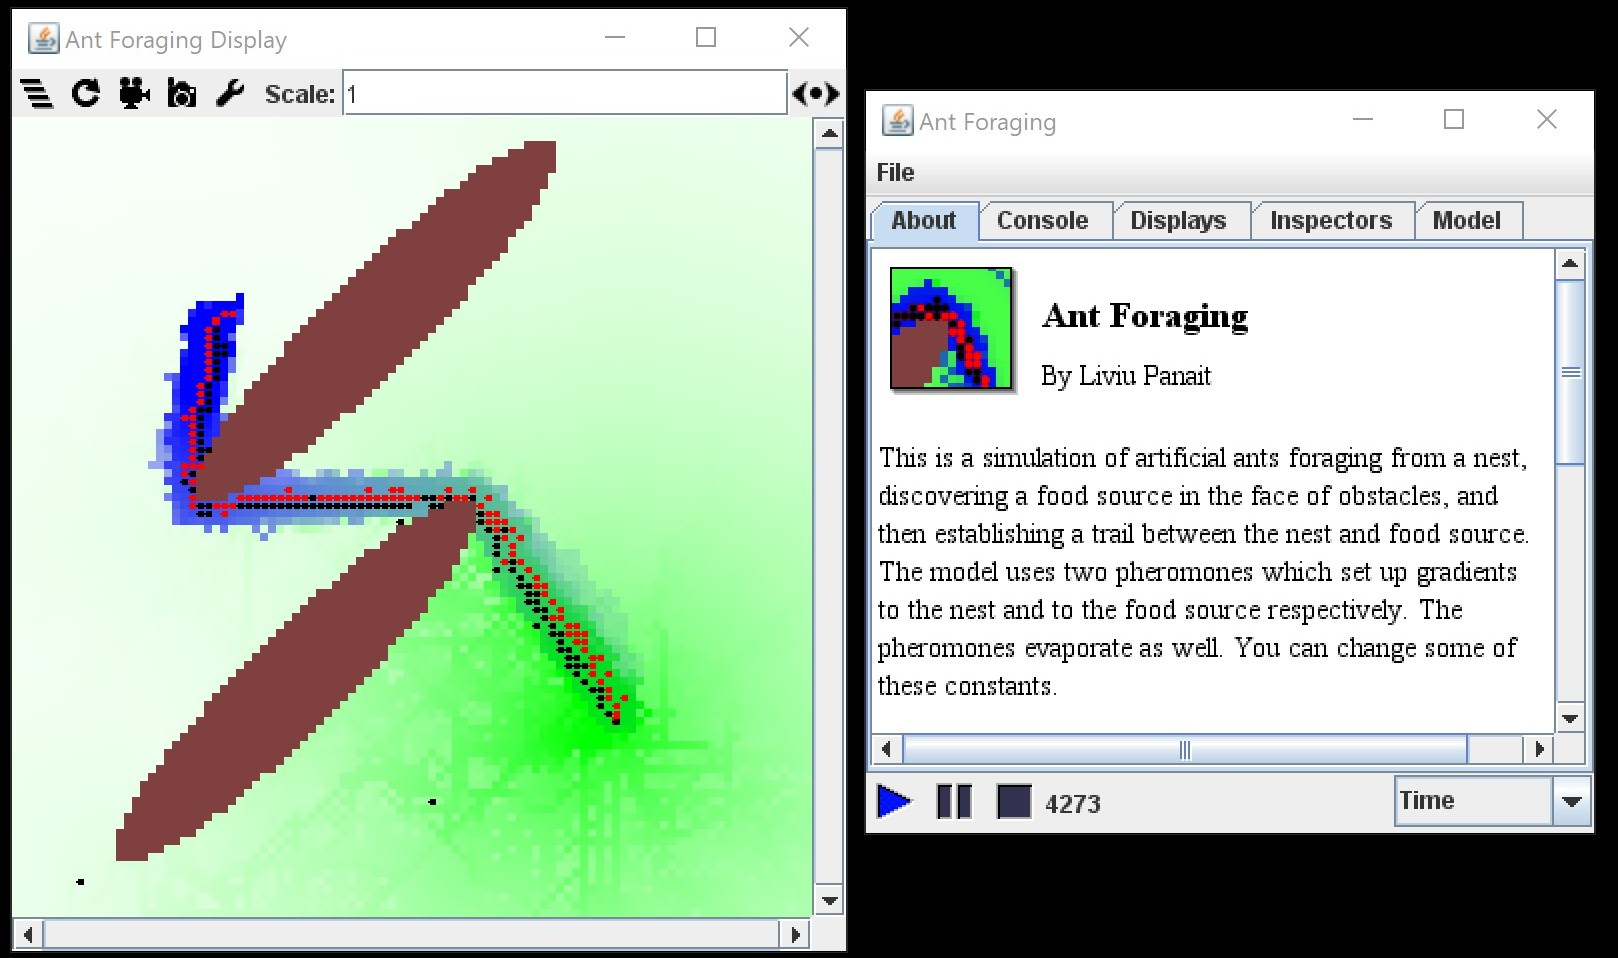
\includegraphics[width=1.0 \columnwidth]{MASON_Ant_Converged.jpg}
	\caption{Convergence of ant in the simulator \citep{Ant_Simulator}}
	\label{fig:MASON_Ant_Converged}
	%\end{center}
\end{figure}

\chapter{Design}
\label{chap:design}
\section{MoSCoW}
\subsection{Must}
\begin{tabular}{|| p{3.5cm} | p{10.5cm} ||} 
	\hline
	Requirements & Description \\
	\hline
	Independent ant movements & Ants must move independently from each other \\
	\hline
	Creating hive & Allow creation of a hive. The hive will be the starting point of all ants belonging to that hive. \\
	\hline
	Static food & Allow creation of static food items on the map. \\
	\hline
	Pheromone types & Contain a pheromone system that allows deposition of pheromone values on the ground. \\
	\hline
	Pheromone evaporation & Deposited pheromones should decrease in concentration overtime in a fixed rate. \\
	\hline
	Obstacle creation & Able to create obstacles that ants can't move on or under \\
	\hline
	Ant births & Able to dynamically generate ants in with a given birth rate \\
	\hline
	Ant death & Ants will die and be removed from the map by probabilistic death rate \\
	\hline
	Pause and play simulation & Allow users to pause the running simulation and replay it multiple times \\
	\hline
	Shows ant data dynamically & Shows ant population and time elapsed on the UI dynamically  \\
	\hline
\end{tabular}

\subsection{Should}
\begin{tabular}{||p{3.5cm} | p{10.5cm} ||} 
	\hline
	Requirements & Description \\
	\hline
	Customisable hive location & The hive location of ants should be customisable on allowed locations on the map. \\
	\hline
	Customisable food location & Food items should be customisable on allowed locations on the map. \\
	\hline
	Customisable global evaporation rate & Rate of evaporation of pheromones can be customised\\
	\hline
	Reset simulation & Allows resetting the simulation with different values \\
	\hline
	Time scaling & Automatically scales the time to reflect realistic values. Allow users to enter actual values for attributes that are connected to time.\\
	\hline
\end{tabular}

\subsection{Could}
\begin{tabular}{|| p{3.5cm} | p{10.5cm} ||} 
	\hline
	Requirements & Description \\
	\hline
	Multiple hives & Allows creation of multiple ant colonies with varying population \\
	\hline
	Customizable terrain & Terrains can be customised by the users by painting pixels on the map \\
	\hline
	Moving food item & Allows creation of food item that moves across the screen \\
	\hline
	Predator & Allows creation of predators that attacks and consumes the ants\\
	\hline
	Customisable individual evaporation rate & Allows customisation of individual evaporation rates \\
	\hline
	Preset ant settings & Provides a list of settings that reflects actual values of ant species \\
	\hline
	Varying ant types & Allows creation of different types of ant within a colony \\
	\hline
	Pheromone data at point & Outputs the pheromone data of a particular point in the map\\
	\hline
	Creation of new pheromones & Allows creation of pheromones with different properties\\
	\hline
\end{tabular}

\subsection{Won't}
\begin{tabular}{|| p{3.5cm} | p{10.5cm} ||} 
	\hline
	Requirements & Description \\
	\hline
	Detailed UI models &  The UI of different items(sprites) in the simulator will not have detailed models and will be represented by simple shapes\\
	\hline
	In-built screen recording & The system will not provide recording features \\
	\hline
	Nupital flight simulation & The system will not simulate the process of nupital flight \\
	\hline
\end{tabular}

\section{Structure of the system}
The system will have different classes assigned with various responsibilities. The \textbf{Display class} will be the creator of the simulator. This class will be called first during execution of the Java executable. This class will create the windows(stages) for the simulator. All information of the simulator such as time, all sprites and are saved in the \textbf{Ant\_Simulator class} shared to other classes when required. After the simulator has been initiated, the \textbf{Menu\_Controller class} will be assigned the ability to run, modify and terminate the simulator. The system was design with a few base classes that the ant simulator inherits from such as Simulator, Sprites and Ground\_Data class. This allows the improves code re-usability if other simulators are to be built in the future. The full class diagram can be found in figure \ref{fig:Full_Class_Diagram} in the appendix.

  The state diagram of individual ants are shown in figure \ref{fig:State_Diagram}. All ants have a lifespan that is set during initialisation of the simulator. Death of ants are calculated by probability, the closer they are towards the lifespan, the higher the chance of death. Dead ants are removed from the simulator through the handler.

\begin{figure}[htb]
	\begin{center}
	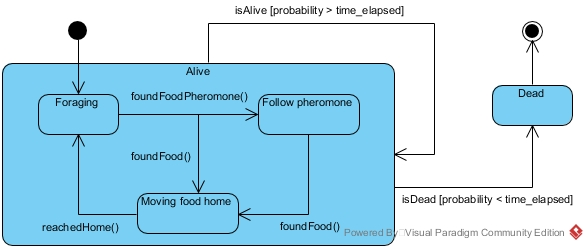
\includegraphics[width=0.8 \columnwidth]{State_Diagram.jpg}
	\caption{State diagram of an Ant}
	\label{fig:State_Diagram}
	\end{center}
\end{figure}


\section{Ant movement AI}
The ants rely on two type of pheromones, home pheromone that is used by ants carrying food to find their way home and food pheromone which is left my ants carrying food and followed by foraging ants to the food source. Aside from pheromones, the ants will also rely on the distance between their location and the hive and will try to move closer to the hive if possible, mimicking the process of path integration \citep{Ant_Path_Integration}.

All ants can move to the 8 potential directions shown in figure \ref{fig:Ant_Direction}. If there isn't any pheromone data found in their surroundings, the ants will move in random directions but they will prioritise the three direction that the ant is in front. 

During analysis of MASON ant simulator and literatures associated, It was found that the the ants in the simulator relies purely on pheromones for navigation  which might result in ants being stuck in in a cyclic movement if the food source is located further away from the hive where surrounding home pheromones may have evaporated or the density of ants are not high enough to ensure navigation back to the hive. Due to this, individual ants are designed to retain a set amount of locations that it has  recently visited and will avoid moving back to the locations unless necessary. 

Algorithm \ref{Algorithm:General} shows the high level movement pattern of ants. Algorithm \ref{Algorithm:Find_Home}, \ref{Algorithm:Home_Pheromone} and \ref{Algorithm:Home_Distance} shows the algorithm used for ants to find their way back to their hive when carrying food. Movement patterns when ants are following food pheromones to food source are similar to following home pheromones back to the hive.

\begin{figure}[htb]
	\begin{center}
	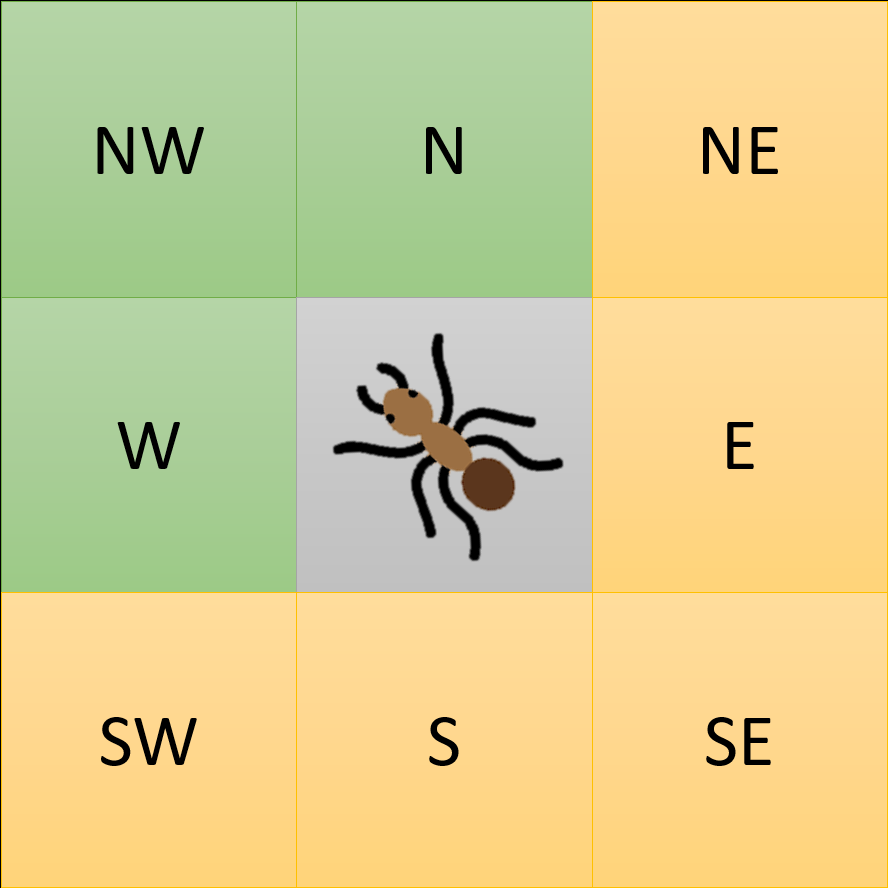
\includegraphics[width=0.35 \columnwidth]{Ant_direction.png}
	\caption{Directions an ant can move to if unobstructed. Ants will prioritise moving towards the three directions in front of them (Ant facing NW). Ant image sourced from \textit{Stockio}}
	\label{fig:Ant_Direction}
	\end{center}
\end{figure}

\begin{algorithm}[th]
\caption{ Ant foraging algorithm } \label{Algorithm:General}
\begin{algorithmic}[1] 
	\If{HasFoodItem}
		\State Find-Direction-Home
	\ElsIf{FoundFoodPheromone}
		\State Follow-Food-Pheromone
	\Else
		\State Random-prioritised-movement
	\EndIf
\end{algorithmic}
\end{algorithm}

\begin{algorithm}[th]
	\caption{ Find-Direction-Home algorithm}  \label{Algorithm:Find_Home}
	\begin{algorithmic}[1]
		\If{Ant reached the hive}
			\State Drop food 
			\State $HasFoodItem \gets False$
		\Else
			\State direction $\leftarrow$ Decide-Direction-Home-With-Pheromone
			\If{direction = NULL}
				\State direction $\leftarrow$ Decide-Direction-Home-Without-Pheromone
			\EndIf
		\EndIf
		\State moveAnt($direction$)
	\end{algorithmic}
\end{algorithm}

\begin{algorithm}[th]
	\caption{ Decide-Direction-With-Pheromone algorithm}  \label{Algorithm:Home_Pheromone}
	\begin{algorithmic}[1]
		\State potential-directions $\leftarrow$ \{ \}
		\While{there's possible directions}
			\If{direction is not blocked}
				\If{direction is closer to hive \& direction wasn't visited recently}
					\If{direction-contains-pheromone}
						\State potential-directions $\overset{+}{\leftarrow}$ direction
					\EndIf
				\EndIf
			\EndIf
		\EndWhile
		\If{potential-directions = NULL}
			\State return NULL
		
		\Else
			\State direction $\leftarrow$ direction-maximum-pheromone$(potential-directions)$
			\State return direction
		\EndIf
	\end{algorithmic}
\end{algorithm}

\begin{algorithm}[th]
	\caption{ Decide-Direction-Without-Pheromone algorithm}
	 \label{Algorithm:Home_Distance}
	\begin{algorithmic}[1]
		\State potential-directions $\leftarrow$ \{ \}
		\While{there's possible directions}
		\If{direction is not blocked}
			\If{potential-directions = NULL \& direction wasn't visited recently}
				\State potential-directions $\overset{+}{\leftarrow}$ direction
			\ElsIf{direction is closer to hive}
				\State potential-directions $\overset{+}{\leftarrow}$ direction
			\EndIf
		\EndIf
		\EndWhile
		\State direction $\leftarrow$ direction-closest-to-home$(potential-directions)$
		\State return direction
	\end{algorithmic}
\end{algorithm}

\chapter{Implementation}
\label{chap:Implementation}
\section{Platform and packages}
The simulator is developed in Java using the IDE \textit{IntelliJ}. Using Java as the development language ensures that the solution can be run on a wide range of Operating Systems while the object-oriented paradigm allows definition of classes that's duplicable and inheritable. This would be beneficial for this project as the simulator involves creation of large amount of objects that are similar structurally but has to behave independently. The UI will also be developed using \textit{JavaFX} as its platform. JavaFX provides the ability to separate UI from the implementation logic using FXML. It allows quick development of simple user interface that can be easily expanded and updated as JavaFX also supports CSS and HTML.

\section{Development stages}
Figures of development stages are included in the appendix

\subsection{Stage 1}
Stage 1 focuses on creation ants that can move and stay within the boundaries and moves randomly with prioritisation of the three directions in front of them. All values in the simulator are preset. Figure \ref{fig:Stage 1} in the appendix shows a screen capture of stage 1 development

\subsection{Stage 2}
Stage 2 implements the ants capability of locating food and brining it back home. During this stage, the ants will rely on path integration and attempt to move closer to the hive on each tick. The distance to the hive is calculated by euclidean distance. This stage focuses on the ants capability of state change.

\subsection{Stage 3}
Stage 3 focuses on pheromone deposition. According to the state the ants is in, they will deposit either home or food pheromone and the pheromones will evaporate at a fixed rate over time. Movement of ants was also modified to rely on pheromones for path finding.

\subsection{Stage 4}
Obstacles was implemented during stage 4. Additional obstacle data was added onto the ground data which is has a unique property that stops ants from moving across or over it. To adapt to it, ant movement algorithm was further expanded to include obstacle avoidance.

\subsection{Stage 5}
Stage 5 involves the implementation of controller window, modifiable values and extra attributes such as birth rate and death rate. Ant movement algorithm was further improved to include local memory to improve the efficiency.

\section{Final product}
\subsection{User interface}
The user interface contains two windows, the simulator window and control window (figure \ref{fig:Main_Simulator}). The simulator window contains all the sprites and will be showing the ant movements when the simulator is initiated. The window responds to mouse clicks and will add the home location and food location during set up and returns the pheromone data at the clicked point when the simulator is running. The control window will provide instructions during setup, prompting the user to select the locations of hive and foods. After the simulation has started, the window provides settings that can be modified and simulator controls. Figure \ref{fig:Location_Selection} and \ref{fig:Main_Simulator} shows the user interface.
\begin{figure}[htb]
	\begin{center}
		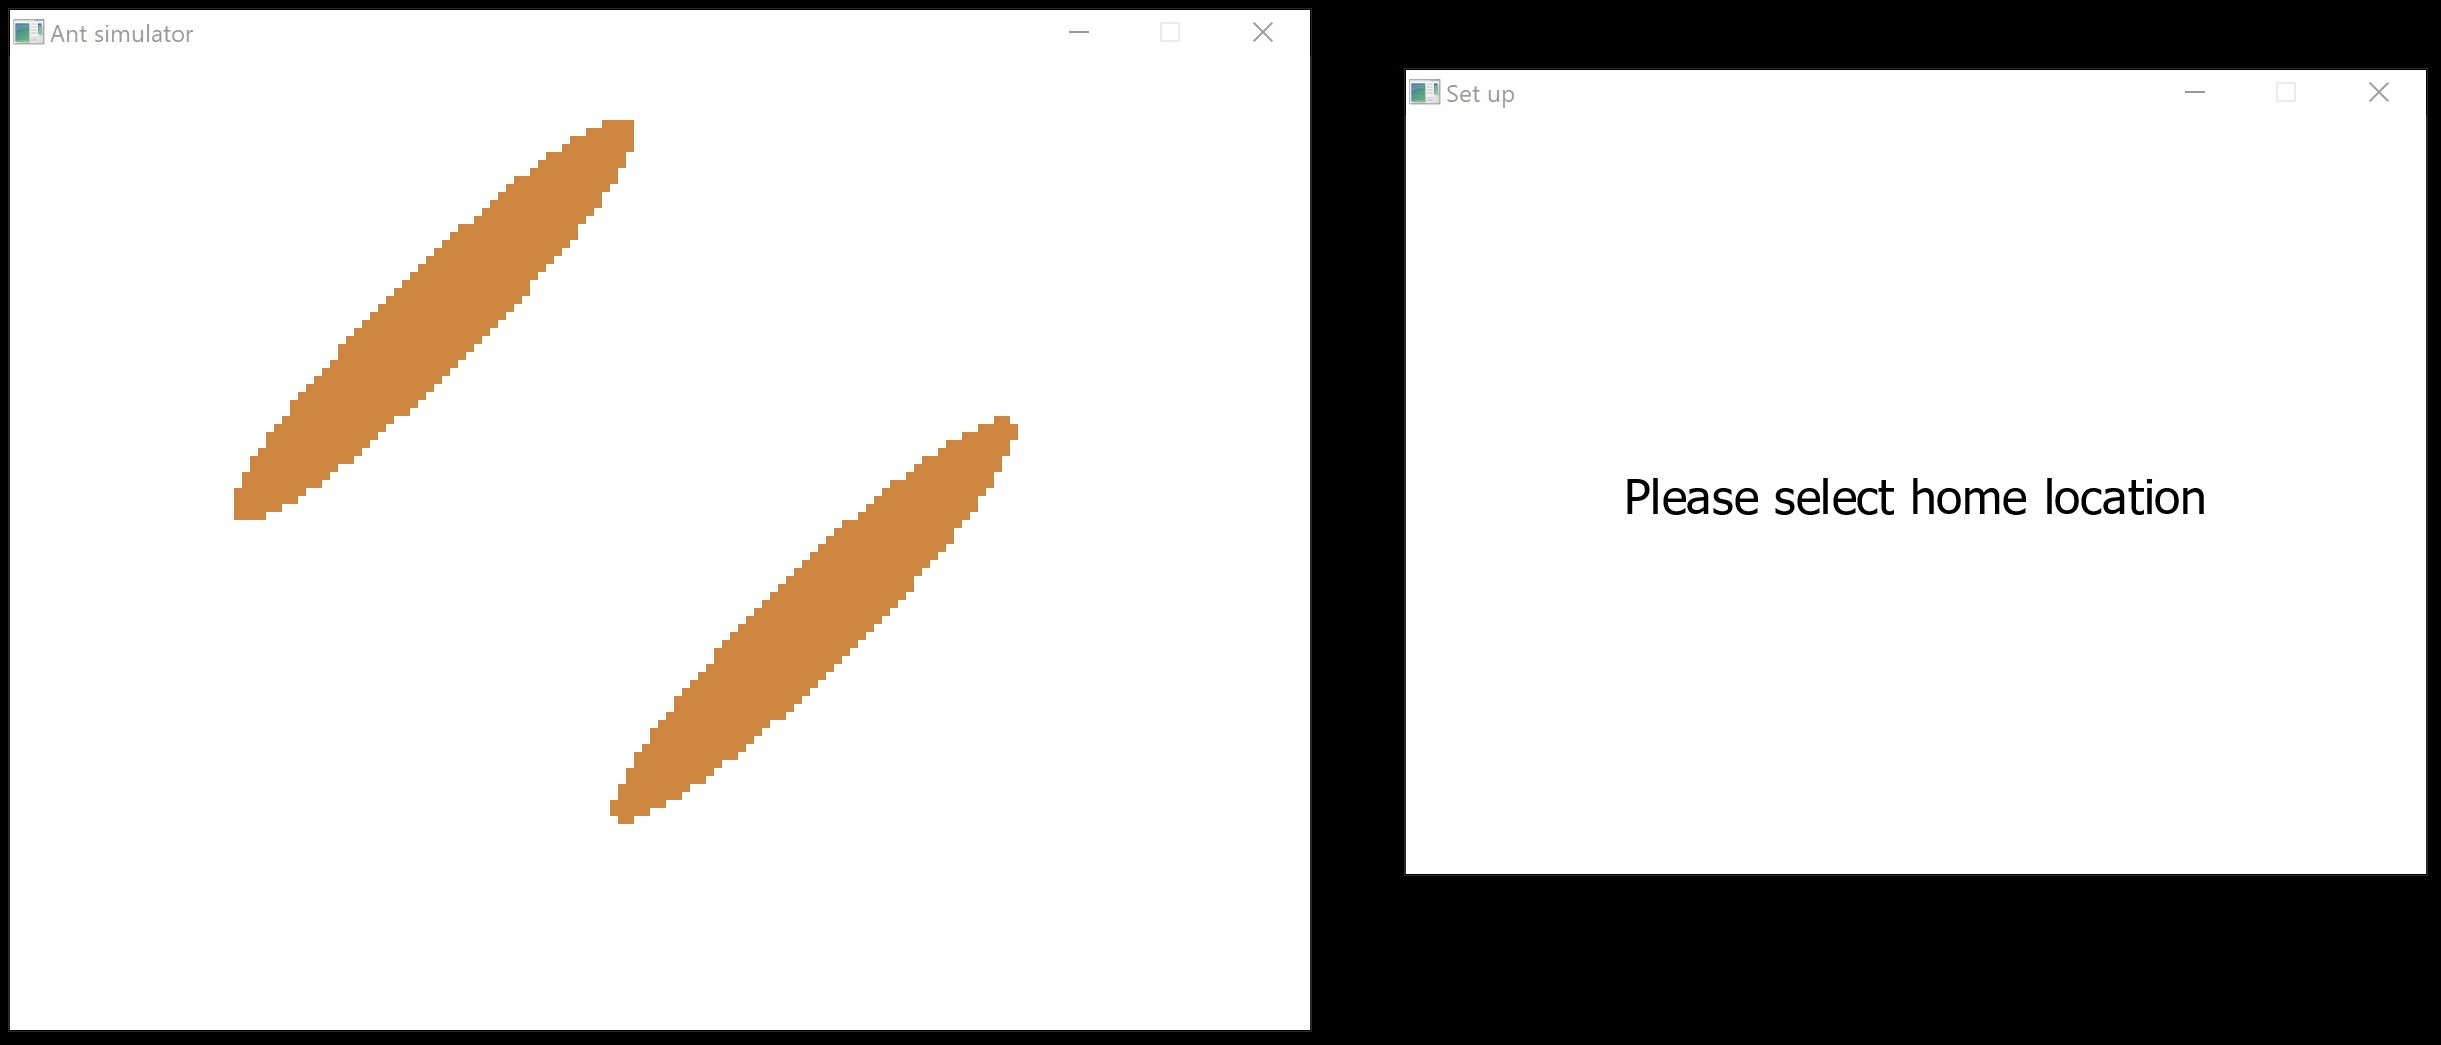
\includegraphics[width=1.0 \columnwidth]{Location_Selection.jpg}
		\caption{Selecting locations for hive and food.}
		\label{fig:Location_Selection}
	\end{center}
\end{figure}

\begin{figure}[htb]
	\begin{center}
		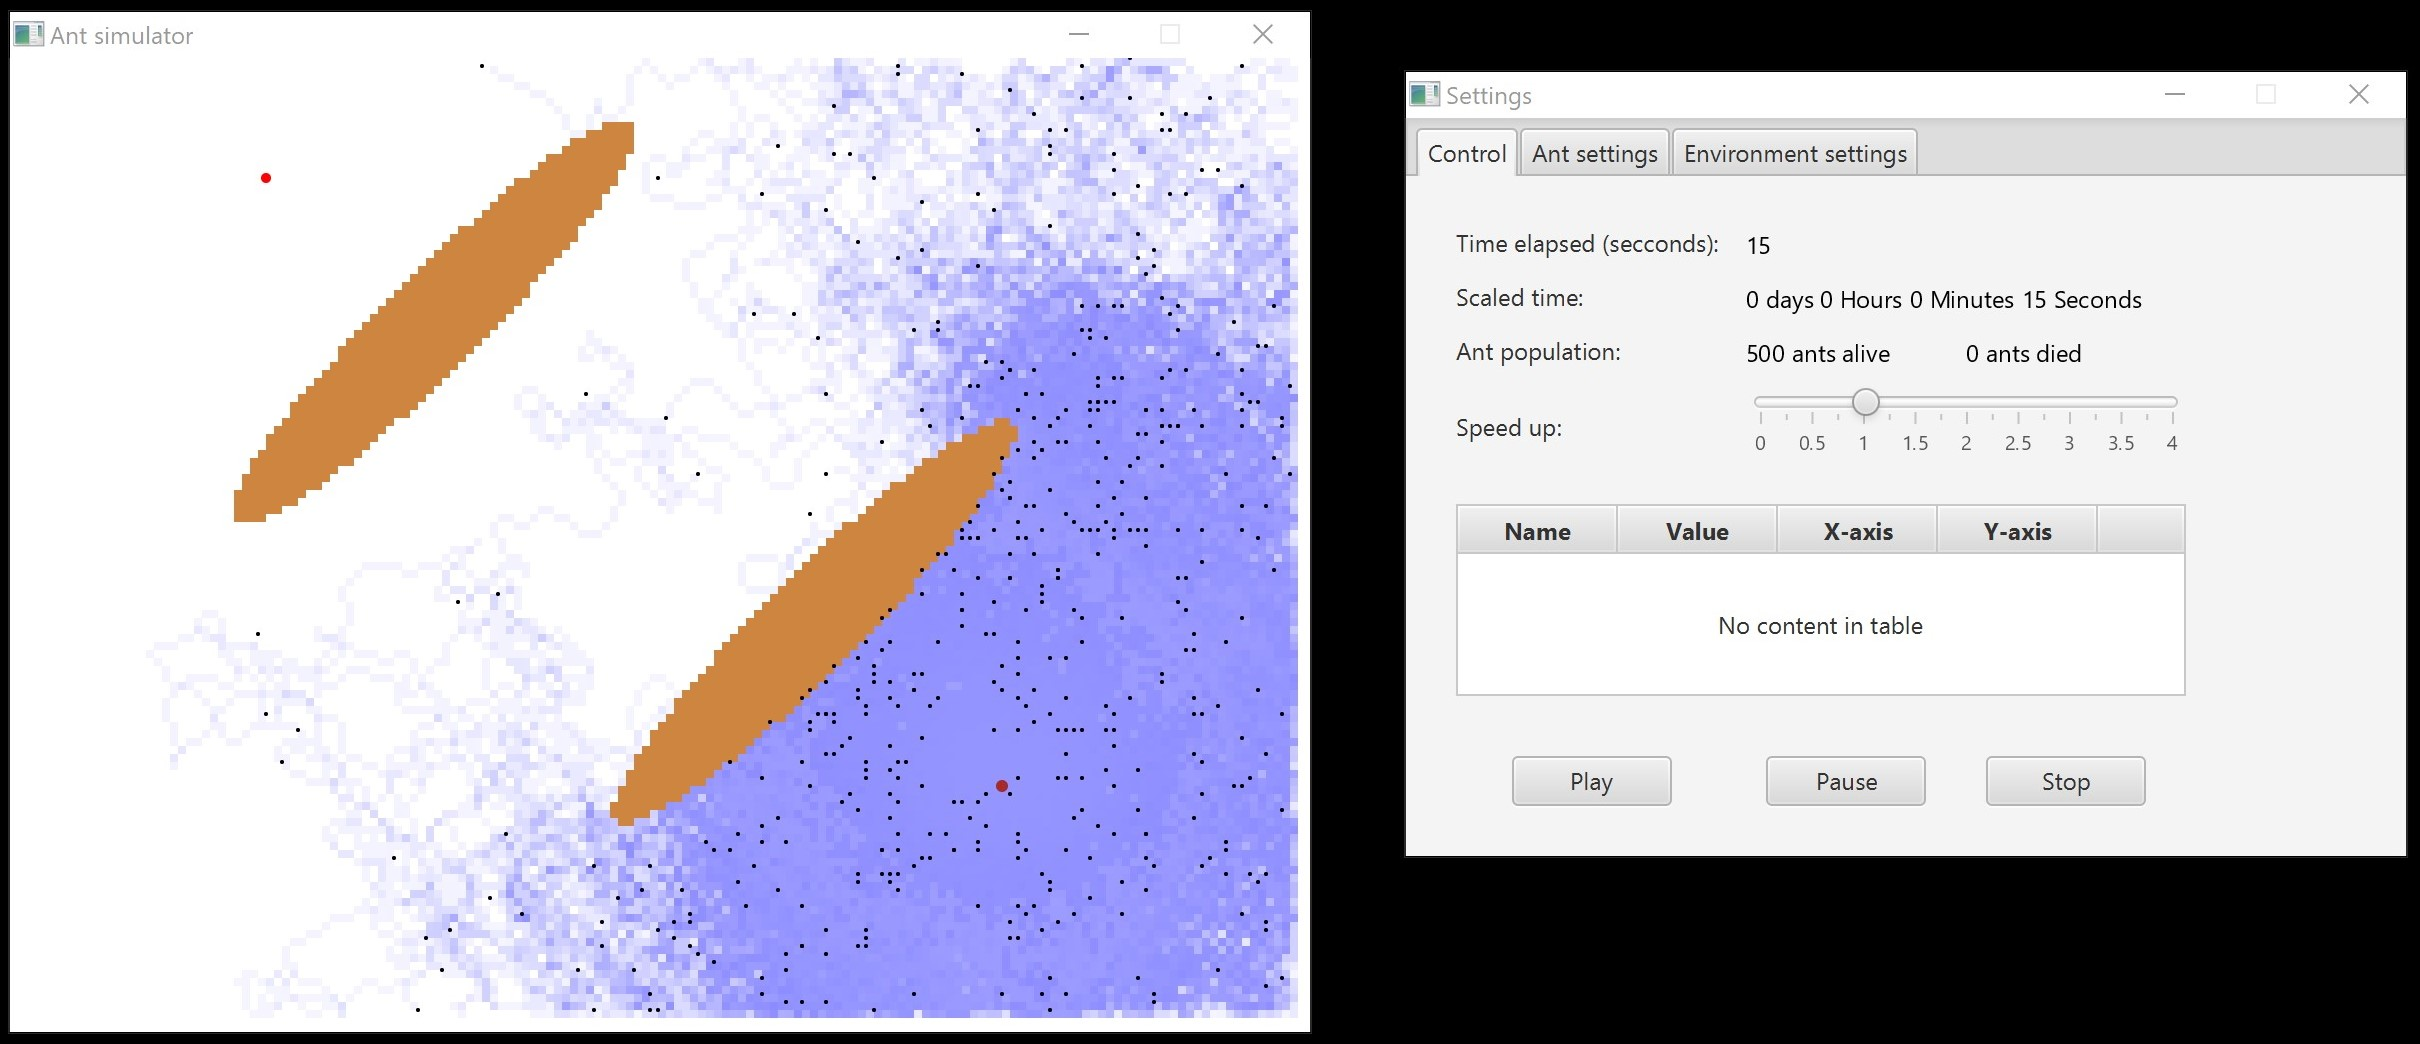
\includegraphics[width=1.0 \columnwidth]{Main_Simulator.jpg}
		\caption{Main UI for the ant simulator. The simulator window is located on the left and the control window is on the right.}
		\label{fig:Main_Simulator}
	\end{center}
\end{figure}


\chapter{Testing}
\label{chap:Testing}
As the design of the static classes are straightforward, testing is conducted heavily towards the end of the development prioritising Dynamic black box and white box testing. Bugs and issue are predicted to be mostly emergent, caused by the ants interaction with its environment.

\section{Unit testing}
For unit testing, values that are passed to and object are checked using console output to print out the values. Values printed out on the console are shown in figure \ref{fig:Ant_Simulator_Values} and \ref{fig:Ant_Values} in the appendix. A test class was also created to test out  new methods and packages before integrating it into the system (Figure \ref{fig:Test_Class}). In these unit tests, expected and unexpected values are entered to the methods to test if the return values are expected.

\section{Integration testing}
Integration testing focuses on parameter passing from the UI to back-end and vice-versa. This is achieved by firstly outputting the values passed from the UI to other classes to the console and checking if the input matches the output. Integration testing was also conducted with each stage of implementation. The simulation was executed a left for a duration to reveal potential bugs with each addition of features. 

\section{User testing}
Three users were selected to conduct black box testing on the finished software. The users were initially not given any information on the software except the main aim and was tasked to interact with the software. Most users managed to utilise the simple function of the software (e.g. pausing and playing) however they struggled with modifying the values. Descriptions of the value were then modified to provide better guidance for the types of input a user can put in. The users were then instructed to complete the tasks listed below:
\begin{itemize}
	\item Speed up the ants movement
	\item Modify the ants settings
	\item Increase the time scale of the simulator
	\item Get the pheromone values of a particular coordinate
\end{itemize} 
All bugs encountered during testing was recorded and fixed after the test.

\chapter{Discussion and Evaluation}
\label{chap:discussion}

From s review of the MoSCoW analysis, the ant simulator has managed to fulfil all the requirements in must and should. It also managed to achieve a requirement in the could section such as obtaining pheromone data at a point on the map. The simulator is able to provide simulations with a range of different values. 

However, during stress testing, the simulator is shown to slow down significantly or freeze when the population of ants goes past 2000. Future improvements could introduce parallel programming for processing of ant movements to allow the simulator to accommodate larger ant populations. Although the ants doesn't show cases of cyclic movement in the tests, there are cases where ants struggle to find a path home. Ants will trace the sides of obstacle when attempting to locate the path home which consumed time and affected the results of when converging to an optimum path. Future improvements can be made to improve the decision making of the ants during movements to include more factors described in chapter \ref{chap:background} to ensure that optimum paths can be found more efficiently. Additionally, some values in the simulator are currently not customisable such as the potency of pheromones and individual rates, future improvements could consider implementing these as customisable values.

Due to the structure simulator was built, this software provides high flexibility when it comes to scaling and reusing. Similar simulators can potentially be built using this software as it's base, providing opportunities for large amount of future work.

\chapter{Conclusion and future work}
\label{chap:conclusion}
This ant simulator provided a simple implementation for running a small scale ant colony that behaves similarly to real life ants. It utilises path utilisation, pheromone trails and visual memory to create an intelligent movement pattern for the ants. The simulator also showcased the interaction of different simplistic agents to complete a task together.

For future work, I intent to to improve the ant path-finding algorithm to better match it's biological counterparts and expanding it's features to accommodate a larger range of values, environments and species.


\bibliographystyle{unsrt}
\bibliography{References}

\chapter*{Appendix A}
\begin{figure}[htb]
	\begin{center}
		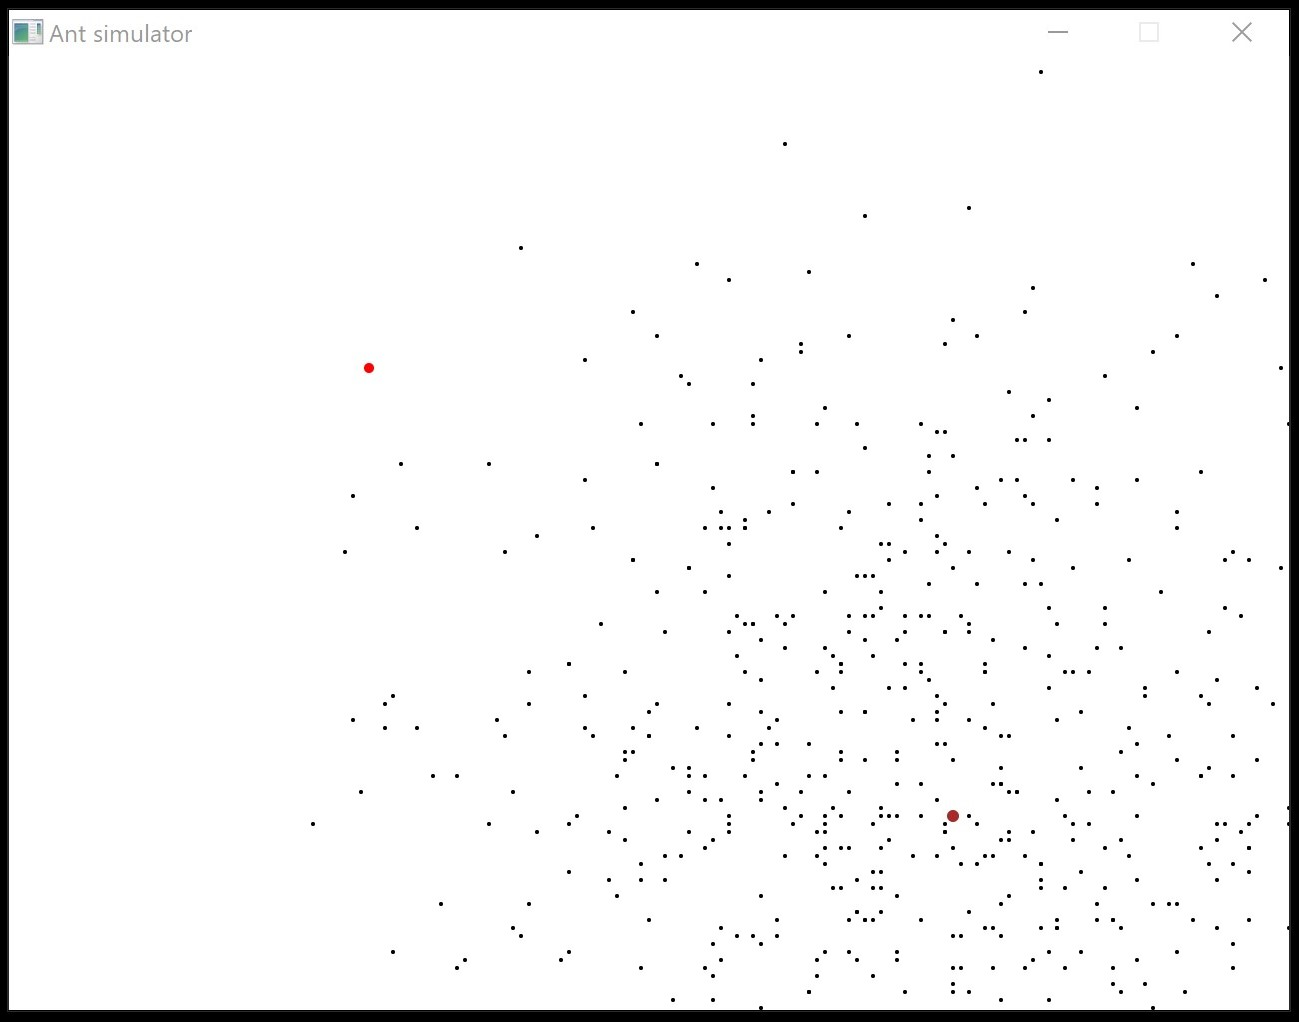
\includegraphics[width=0.65 \columnwidth]{Stage_1.jpg}
		\caption{Stage 1 of development. The black dots shows the ants and the red dots are the hive and food.}
		\label{fig:Stage 1}
	\end{center}
\end{figure}

\begin{figure}[htb]
	\begin{center}
		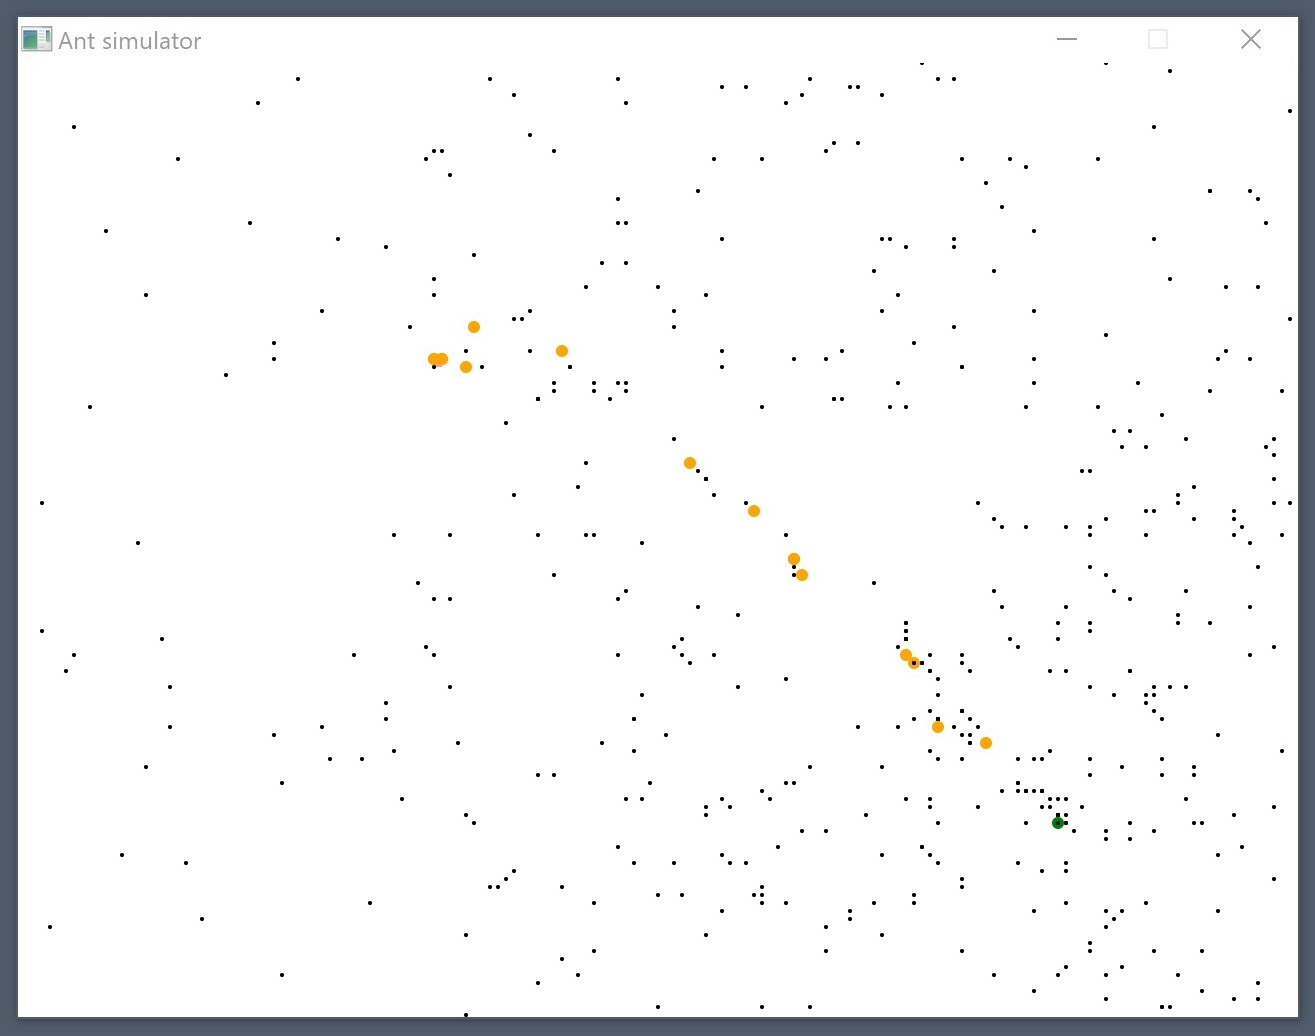
\includegraphics[width=0.65 \columnwidth]{Stage_2.jpg}
		\caption{Stage 2 of development. Ants are able to locate food and bring it back to the hive.}
		\label{fig:Stage 2}
	\end{center}
\end{figure}

\begin{figure}[htb]
	\begin{center}
		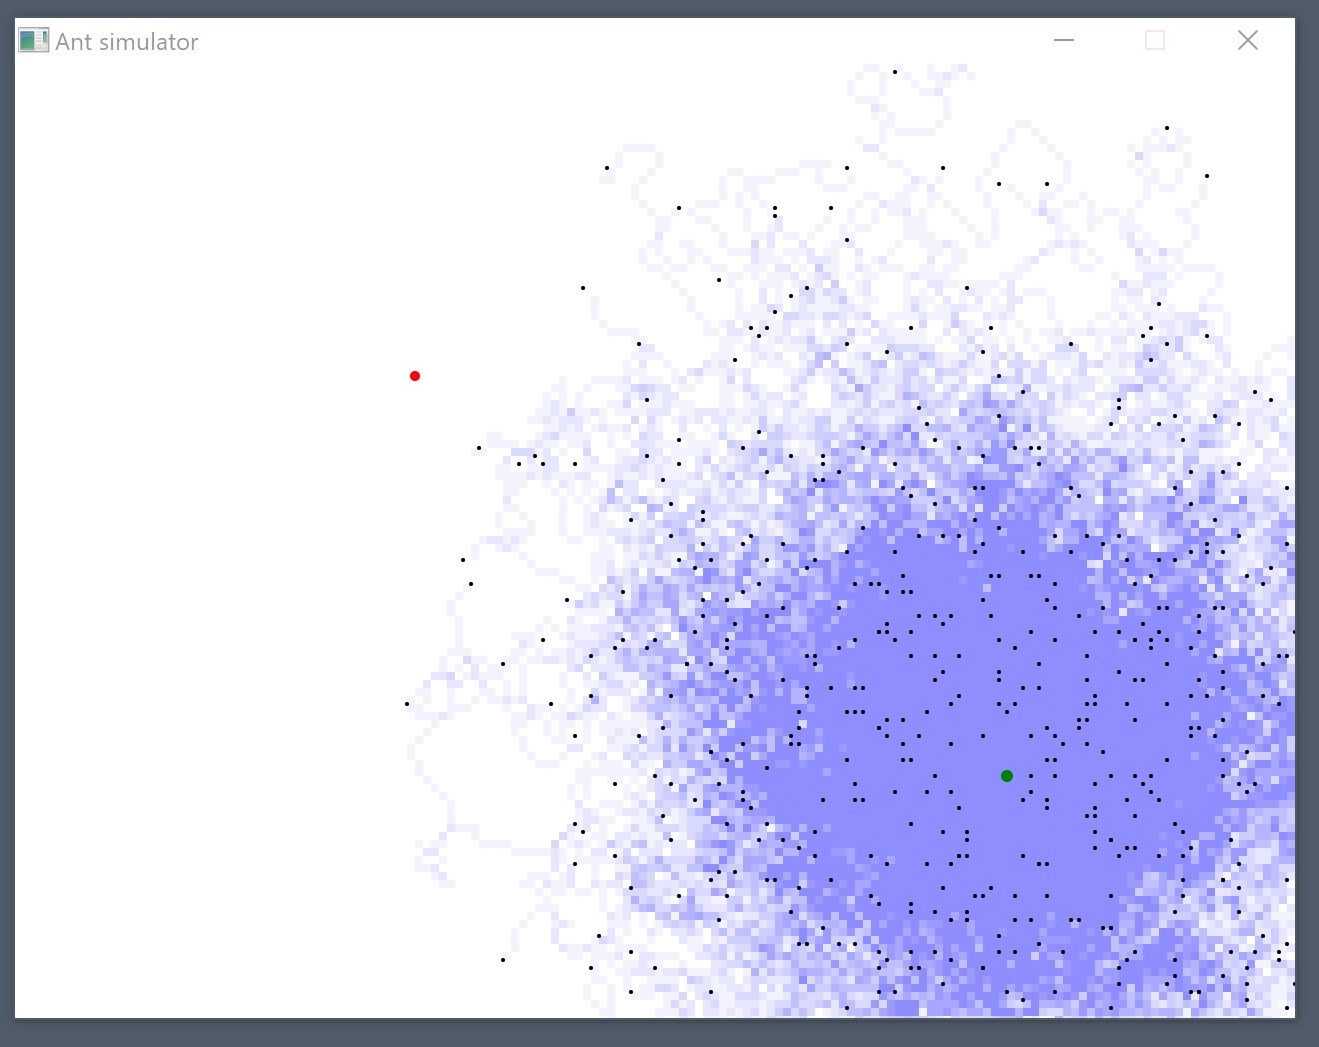
\includegraphics[width=0.65 \columnwidth]{Stage_3.jpg}
		\caption{Stage 3 of development. Ants leave pheromones while foraging.}
		\label{fig:Stage 3}
	\end{center}
\end{figure}

\begin{figure}[htb]
	\begin{center}
		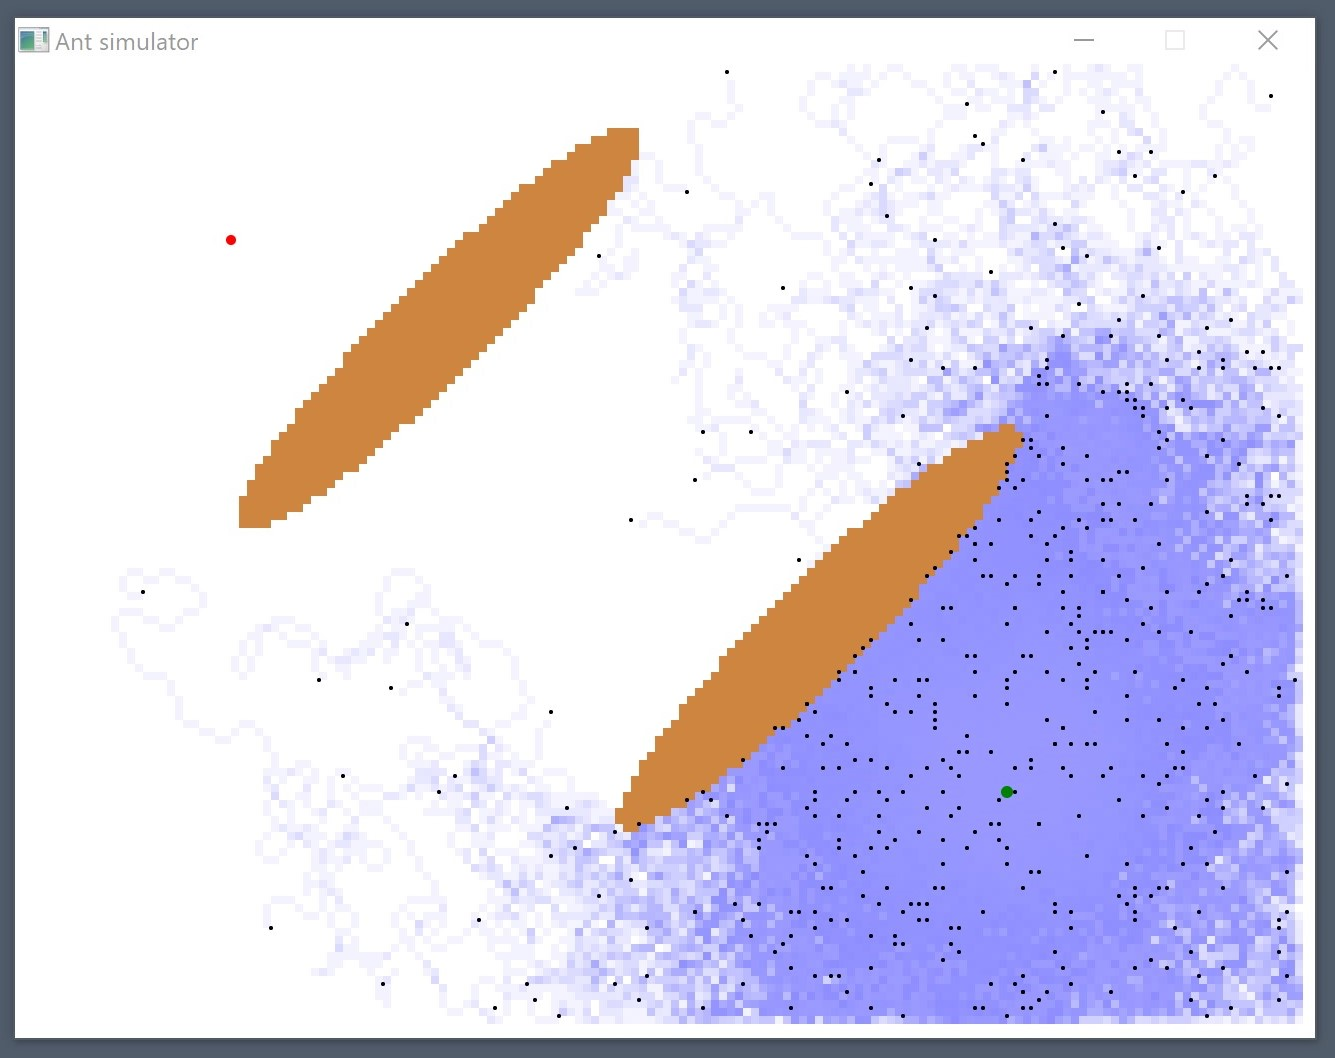
\includegraphics[width=0.65 \columnwidth]{Stage_4.jpg}
		\caption{Stage 4 of development. Ants movement involves avoiding obstacles.}
		\label{fig:Stage 4}
	\end{center}
\end{figure}

\begin{figure}[htb]
	\begin{center}
		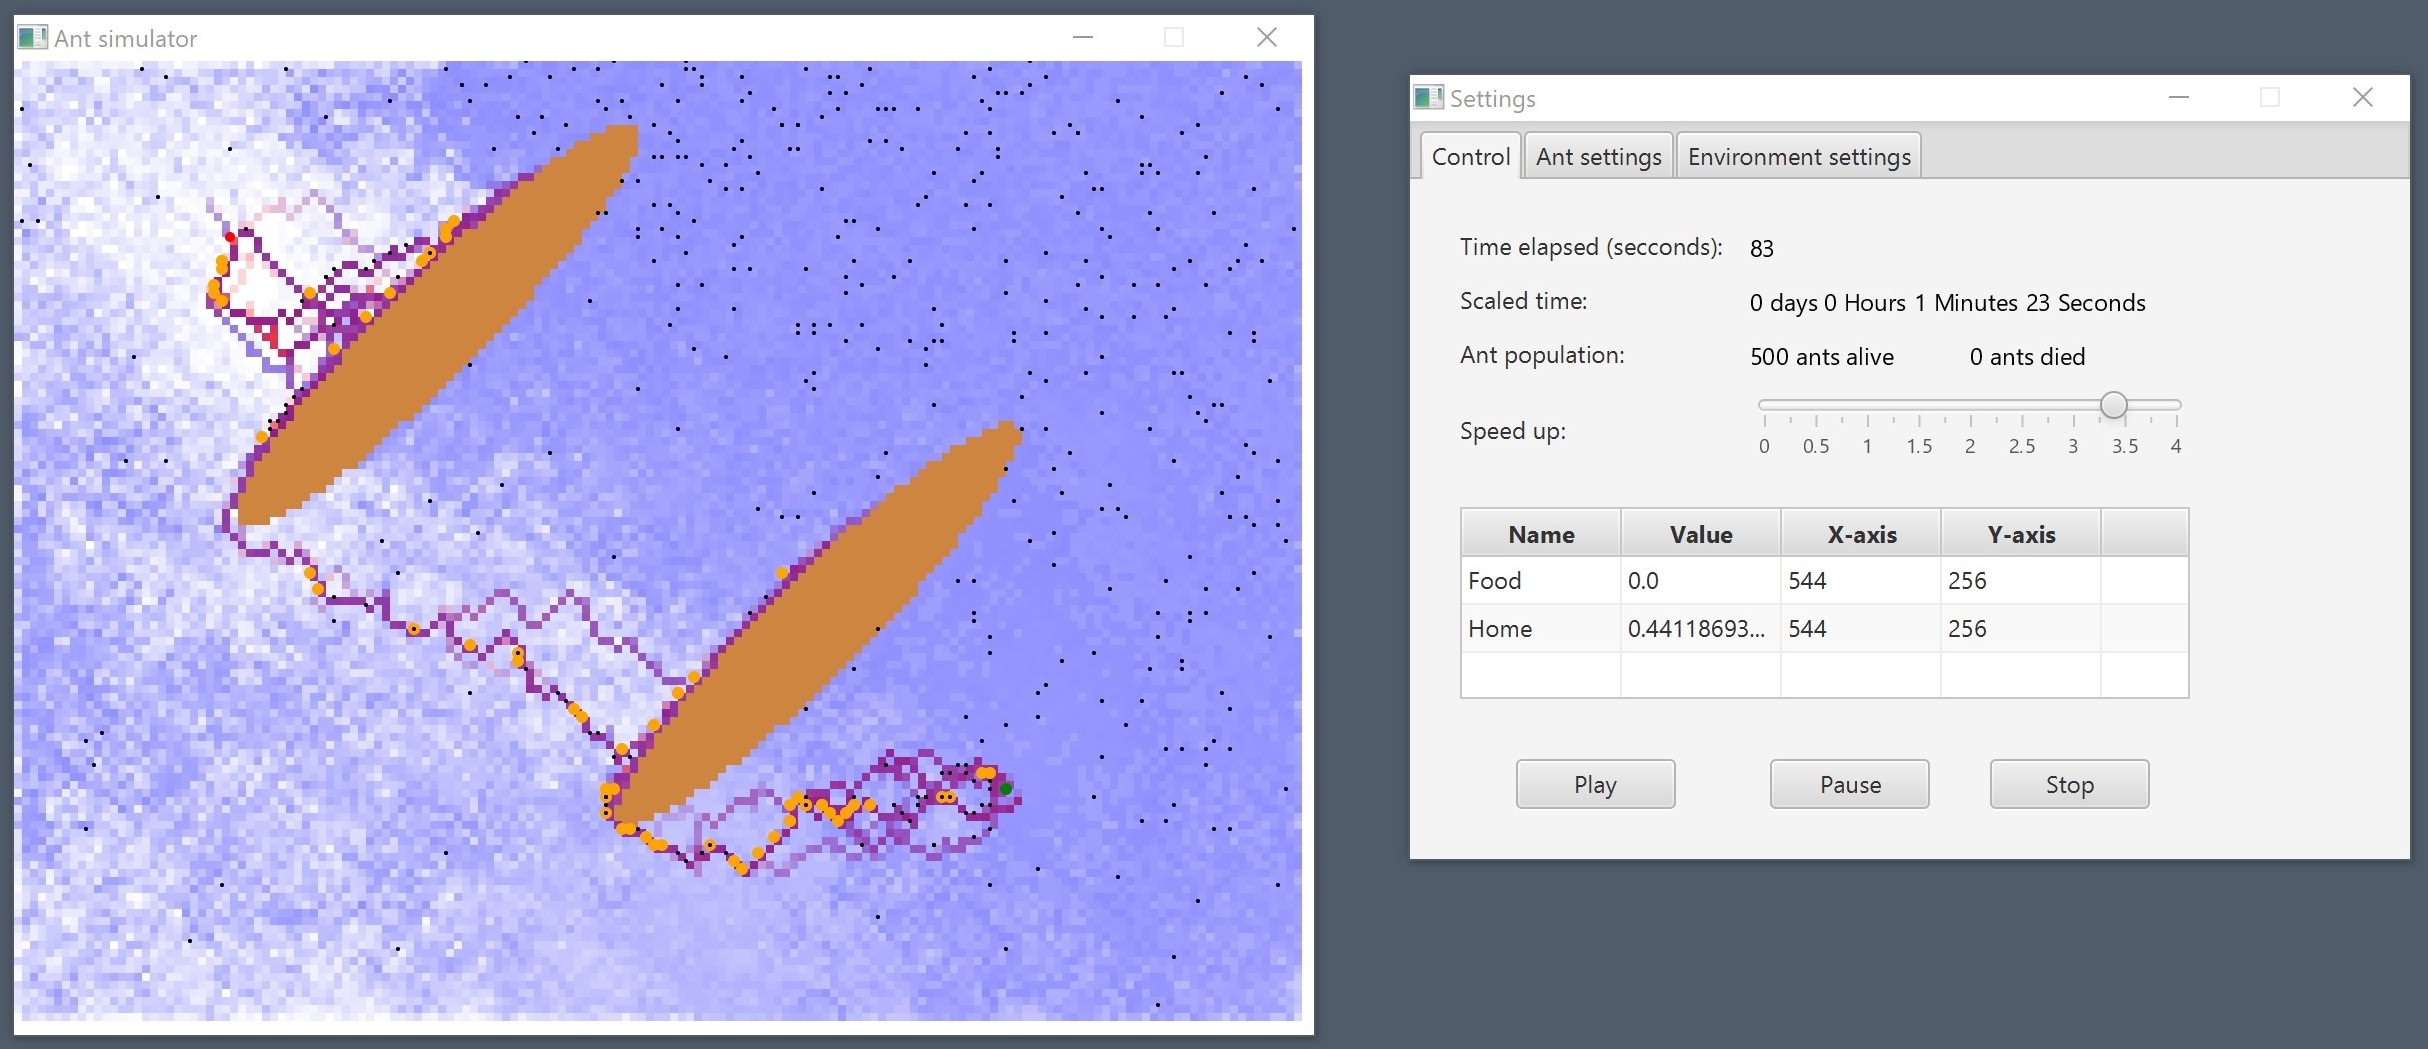
\includegraphics[width=1.0 \columnwidth]{Stage_5.jpg}
		\caption{Stage 5 of development. Implementation of control UI and improving ant path-finding.}
		\label{fig:Stage 5}
	\end{center}
\end{figure}

\begin{figure}[htb]
	\begin{center}
		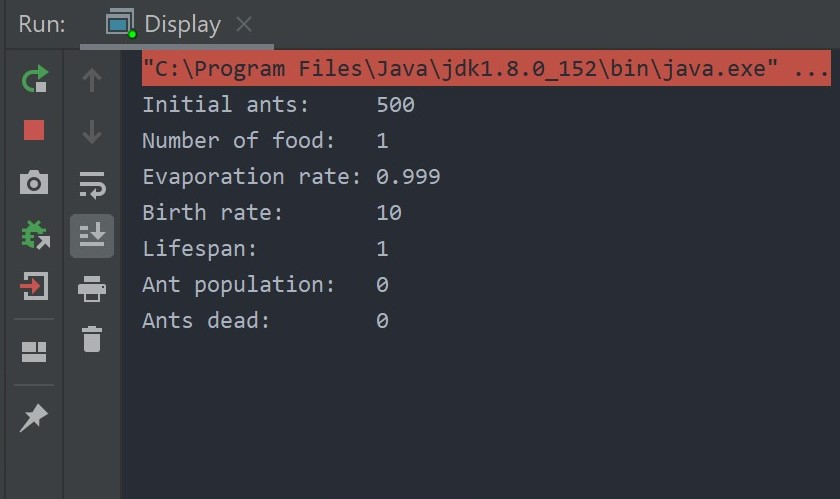
\includegraphics[width=0.6 \columnwidth]{Ant_Simulator_Values.jpg}
		\caption{Values added into the ant simulator printed out to the console}
		\label{fig:Ant_Simulator_Values}
	\end{center}
\end{figure}

\begin{figure}[htb]
	\begin{center}
		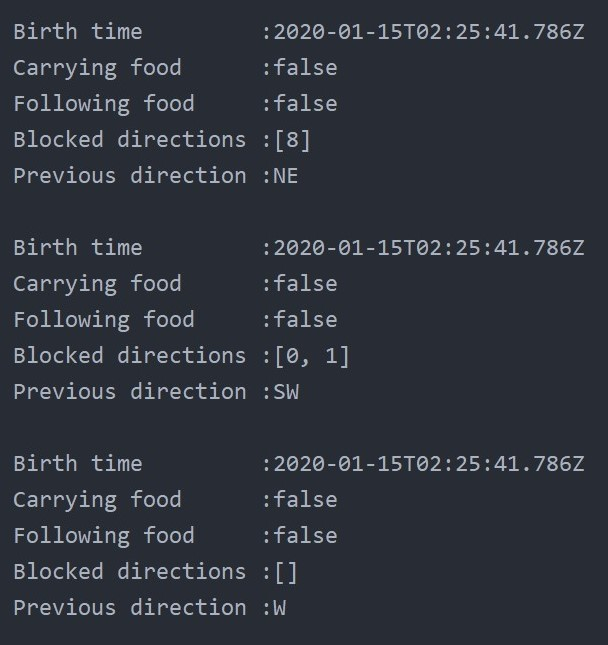
\includegraphics[width=0.6 \columnwidth]{Ant_Values.jpg}
		\caption{Values added into the ants printed out to the console}
		\label{fig:Ant_Values}
	\end{center}
\end{figure}

\begin{figure}[htb]
	\begin{center}
		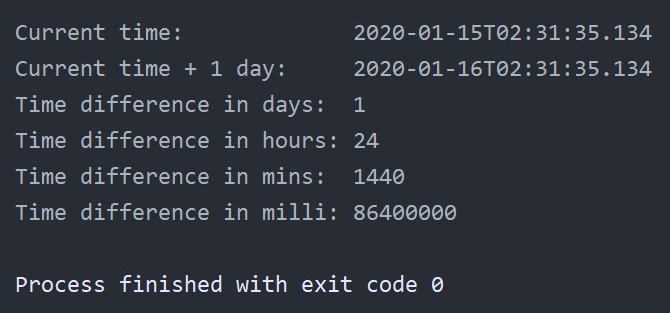
\includegraphics[width=0.6 \columnwidth]{Test_Class.jpg}
		\caption{Using the test class to test the \textit{Instant} and \textit{Duration} class}
		\label{fig:Test_Class}
	\end{center}
\end{figure}


\begin{sidewaysfigure}
	\begin{center}
		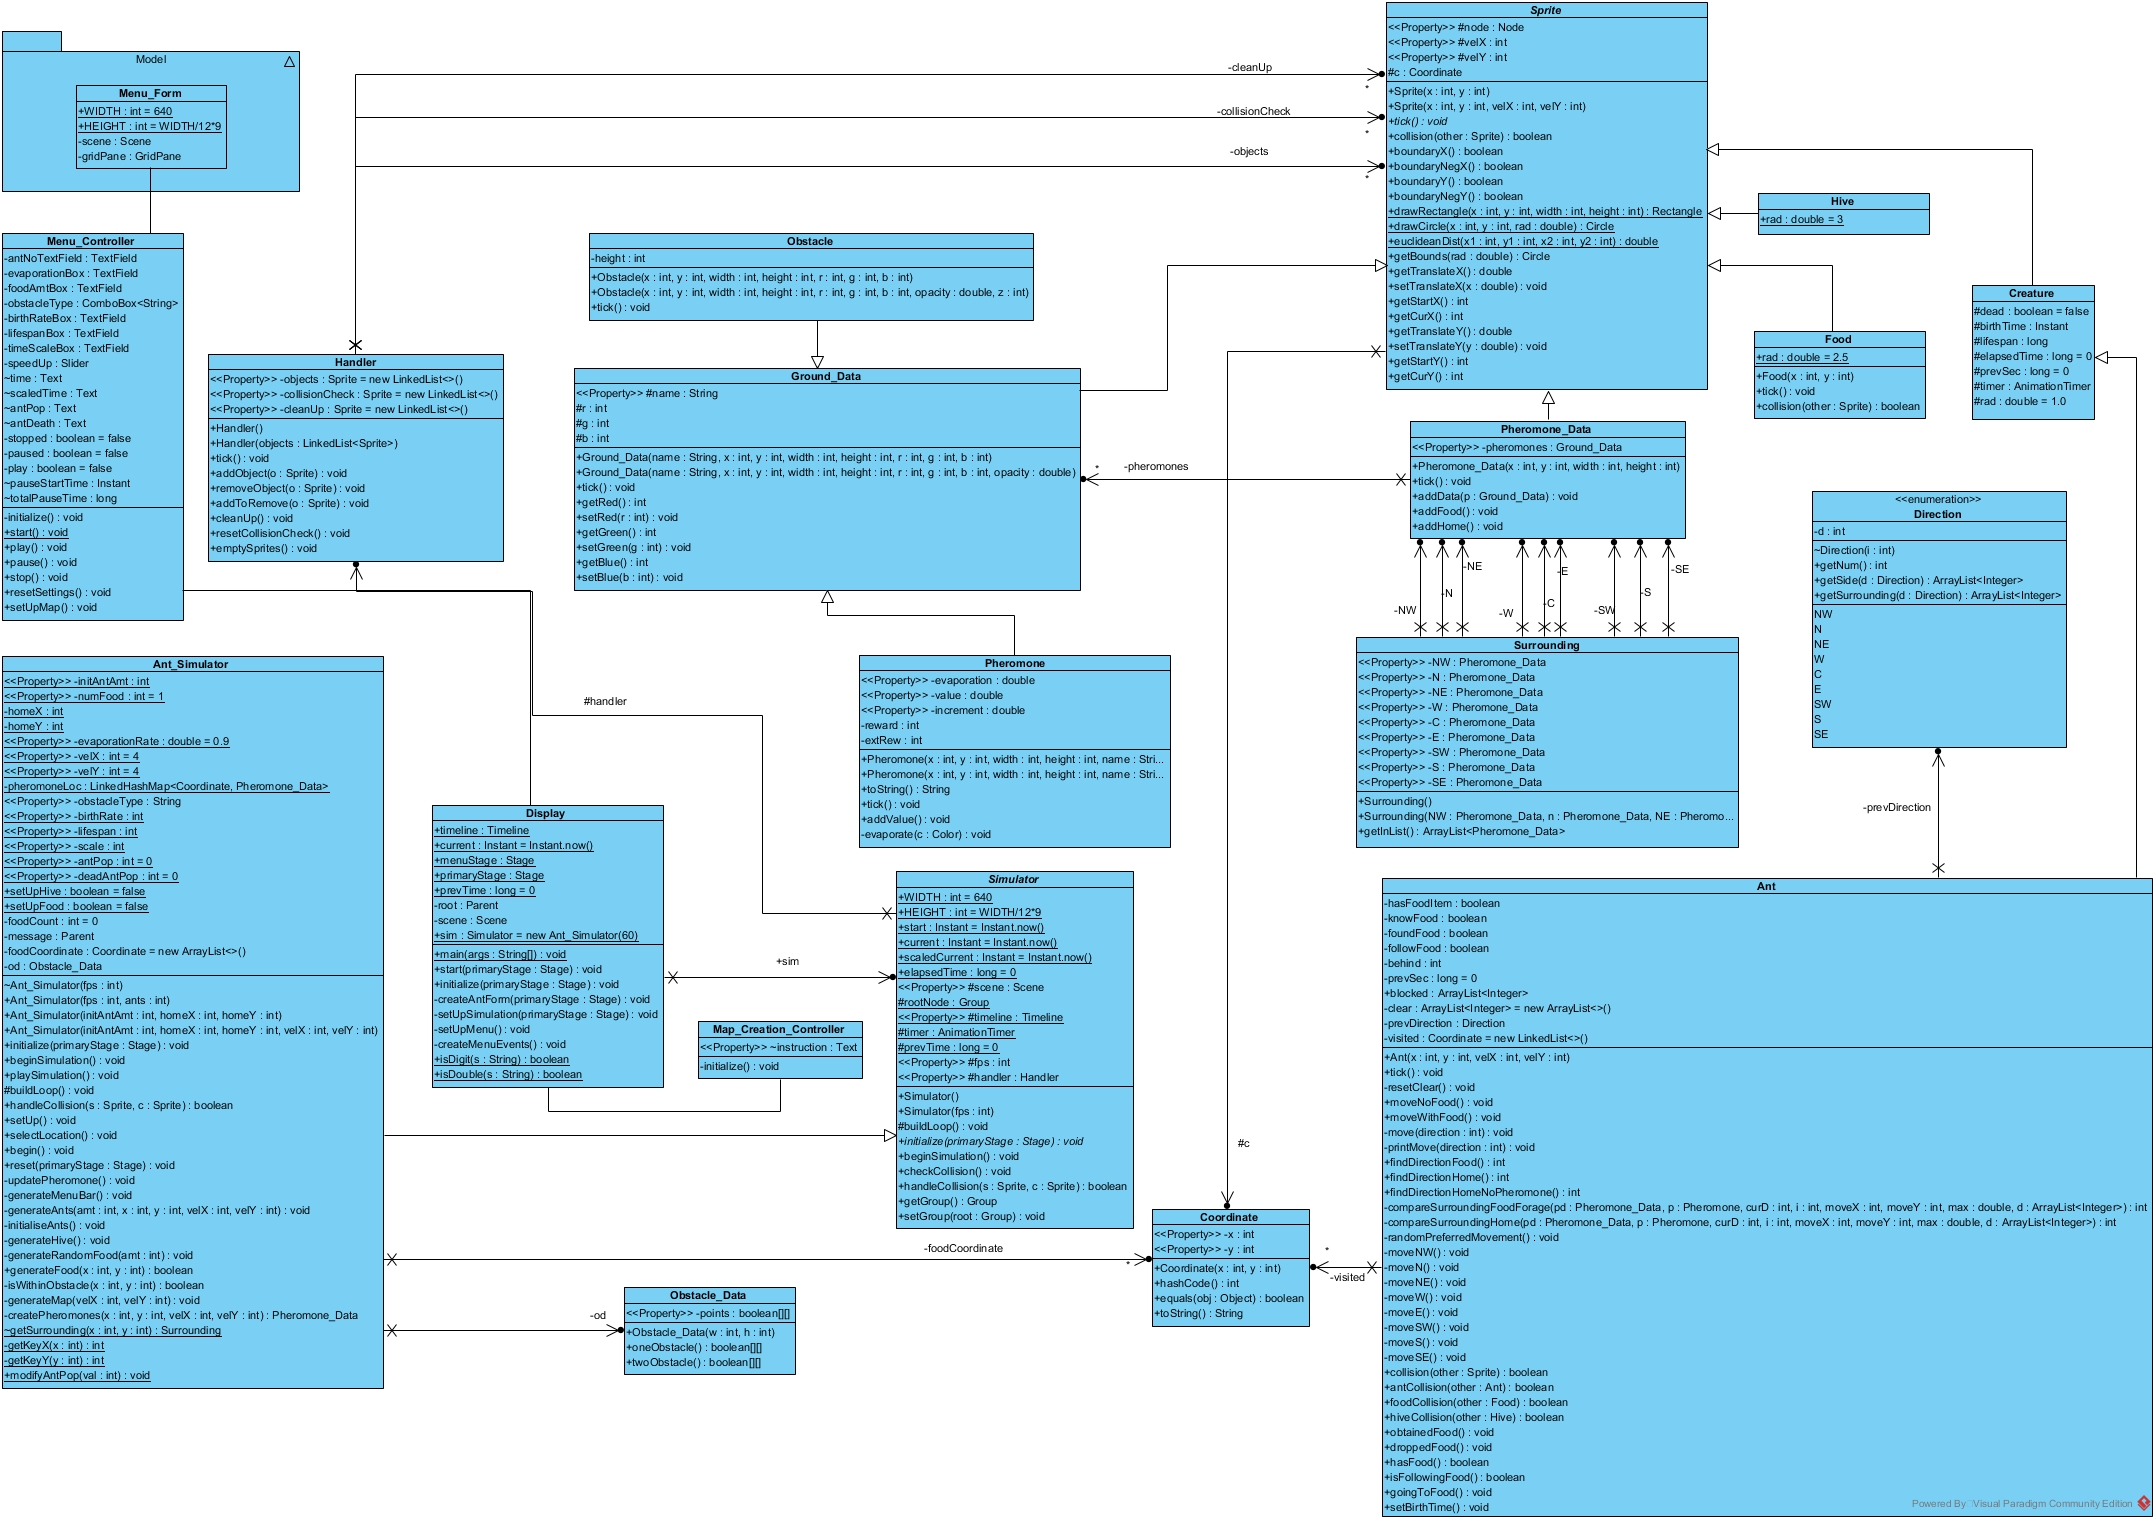
\includegraphics[width=1.0 \columnwidth]{Full_Class_Diagram.jpg}
		\caption{Full class diagram of the Ant simulator}
		\label{fig:Full_Class_Diagram}
	\end{center}
\end{sidewaysfigure}

\end{document}

